%\documentclass[11pt,letterpaper,oneside]{article}
\documentclass{article}
%%%% Conditional for including/excluding answers
\newif\ifanswers
\answerstrue %
\answersfalse % comment out to hide answers

\usepackage{Sweave}
\usepackage{moreverb}
\usepackage{amsmath}
\usepackage{graphicx}
\usepackage{verbatim}
\usepackage{alltt}
\usepackage{moreverb}
\usepackage{enumitem}

\usepackage[latin1]{inputenc}
\newcommand\bcdot{\ensuremath{%
  \mathchoice%
   {\mskip\thinmuskip\lower0.2ex\hbox{\scalebox{1.5}{$\cdot$}}\mskip\thinmuskip}}%
   {\mskip\thinmuskip\lower0.2ex\hbox{\scalebox{1.5}{$\cdot$}}\mskip\thinmuskip}%        
   {\lower0.3ex\hbox{\scalebox{1.2}{$\cdot$}}}%  
   {\lower0.3ex\hbox{\scalebox{1.2}{$\cdot$}}}%
}
\title{The Statistics of LSTM Networks\\ \textit{Adding Clarity to Deep Black-Boxed Models}}
\author{Chris Sweeney 18.S096 Final Project}
\date{Spring 2018}
\begin{document}
\input{18S096-concordance}
\maketitle

\section{Abstract}
Statistical models for analyzing and predicting sequential data have been investigated thoroughly in the last half century. Through drivers like stock market forecasting and modeling human language, a lot of money has been put into creating sophisticated models for time series analysis. However, these models are all derived from a small set of linear processes that fail to perform when modeling complicated sequential data. Interestingly, in the last decade, Recurrent Neural Networks, especially using Long Short Term memory (LSTM) blocks, have seen a lot of success in out-performing traditional sequential statistical models. Unfortunately, too many researchers accept these networks as black box models, and fail to deliberately study the statistics of these LSTM networks. This work will lay out a statistical framework for these LSTM networks, and compare them to more traditional statistical models.

\section{Introduction}
Modeling sequential data has been framed in countless ways, from regression to Hidden Markov Models (HMMs) to Recurrent Neural Networks, and finally to LSTM networks. Each successive scheme for constructing sequential models introduces more complexity and often results in misuses of the models. In section 3 we develop a framework for understanding traditional statistical models like regression and HMMs. We then transition to Deep Models like Recurrent Neural Networks (RNN). In section 4, we provide some transparency into LSTM networks. Finally, in section 5, we evaluate regression and LSTM models' performances on known stationary processes, and compare the pros and cons of each technique. \\

\noindent There are so many ways to analyze and work with time series data. Here are just several examples.\\
\begin{itemize}
  \item Sequence Forecasting
  \item Sequence Classification
  \item Sequence to Sequence 
  \item Anomoly detection
  \item Clustering
\end{itemize}

\noindent For most of the paper, we will focus in on modeling time series from the perspective of forecasting for its simplicity of evaluation, but the analysis for the underlying models carry over to other types of sequential analysis.

\section{Statistics Overview}

\subsection{Regression}
\subsubsection{Overview}
For time series analysis, regression can be thought of as using empirical risk minimization to fit a stateless, linear model to the data. This empirical risk minimization is often posed as minimizing a least squares criterion on observations of a time varying process. A linear combination of these observations and stochastic terms are used to model the movement of the time series process.
We first look at the regression model for a uni-variate time series.\\

  \indent given n observations 1,2...,n of a time series\\
  \indent response variable $y_i$  for i= 1,2...,n (after observations for causal systems)\\
  
  \indent p Explanatory (independent) variables \\
  \indent $xi = (x_{i,1}, x_{i,2}, . . . , x_{i,p})^T, i = 1,2,....n$ \\

\noindent With the General Linear Model: For each case i, the conditional distribution $P(y_i|x_i)$ is given by\\

  \indent $y_i = \hat{y_i} + \epsilon_i$\\
  \indent where $\hat{y_i} =  \beta_1x_{i,1} + \beta_2x_{i,2} + · · · + \beta_Lx_{i,n}$\\

\noindent For regression, the process of fitting a statistical model (finding $\beta_i$) ususally goes as follows.
\begin{enumerate}
  \item Propose the model, choose response, explanatory variables and error terms
  \item Specify judgment criterion
  \item Characterize the best estimator and apply it to the given data
  \item If necessary modify model and/or assumptions and go to (1)
\end{enumerate}

\subsubsection{Model Architecture Analysis}
There is much transparency and introspection into the regression model in this process. One has to explicitly define the model, and thus has a notion of what the parameters in the model are looking for. For example, when modeling time series data for prediction, a high weight on a certain lagged observation suggests statistical significance of that lag term. 

\subsubsection{Model Fitting and Evaluation Analysis}
Probably the best feature of regression is its transparency to the process of fitting parameters to the model. Learning a regression model with the classic Least Squares criterion is creating a Linear Minimum Mean Squared Estimator, that has one defining property: its residual error is orthogonal to the space spanned by the basis of the explanatory variables. This turns out to give the Linear Minimum Mean Squared Estimator a transparent solution.\\

\noindent We now go through a brief overview of fitting parameters for a autoregression model.\\

\noindent For an L lag term uni-variate time series model on zero-meaned process x[n], with linear basis, let y be the forecasting prediction x[n+1]:\\

\indent $y = \beta_0 + \beta_1*x[n] +...+ \beta_n*x[n-L]$ \\

\noindent From orthogonality, where $(y- \sum_{j=1}^{L}\beta_jx_j)$ is the residual error.\\

\indent $E[(y- \sum_{j=1}^{L}\beta_jx_j)x_i] = 0$ for all (n-L)<=i<=n\\

\noindent This statement is equivalent to the following matrix formulation given $\gamma$ is the relative lag terms for predicting x[n+1]\\

$y = x[n+1] = X\beta = $\\
\[
\begin{bmatrix}
    \gamma_{1}       & \gamma_{2} & \gamma_{3} & \dots & \gamma_{L} \\
    \gamma_{2}       & \gamma_{3} & \gamma_{4} & \dots & \gamma_{L+1} \\
    \vdots & \vdots & \vdots &\vdots &\vdots\\
    \gamma_{n}       &  \gamma_{n-1} & \gamma_{n-2} & \dots & \gamma_{n-L}
\end{bmatrix}
\begin{bmatrix}
  \beta_1\\
  \beta_2\\
  \vdots \\
  \beta_L
\end{bmatrix}
=
\begin{bmatrix}
  y_1\\
  y_2\\
  \vdots \\
  y_L
\end{bmatrix}
\]

\noindent The $\beta$ matrix can be solved in closed form from the normal equations $(X^TX)^{-1}X^Ty$

\noindent This is a pretty beautiful result given that so much of optimization deals with nasty non-convexity. As we will see with LSTM networks later, there is not a clear description of the method for fitting parameters.

\subsection{Hidden Markov Models}
\subsubsection{Overview}

Hidden Markov Models (HMMs) approach sequential modeling in a bayesian way that is less dependent on empirical modeling of observations and more concerned with keeping track of a hidden state that governs the model. Various priors for this hidden state allow more flexibility in modeling sequential data, however, it makes the model less understandable. Unfortunately, HMMs are often less useful for time series forecasting, but its analysis will prove useful for explaining LSTM networks.\\

\noindent In regression, we empirically fitted parameters to observations of a sequential process. Now, rather than statically weighing discrete observations, HMM models the movmement of underlying state for the time series process. This idea of modeling a sequential process dynamically rather than a set of distinct observations, like in regression, makes a much more powerful model. However, this complicates optimizing parameters as one now has to keep track of an additional hidden state and how it evolves. (In Recurrent Deep Learning, you have update parameters with respect to these hidden states, known as back propagation).\\

\noindent In HMMs, movement underlying sequential data is described as Markov Chain with observations of the time series at each time step. For hidden state $X_i$ and an observation of uni-variate time series $Y_i$\\

\indent$(X_1,Y_1)\Leftrightarrow (X_2,Y_2)\Leftrightarrow...\Leftrightarrow (X_n,Y_n)$ \\

\noindent Using markov assumption the joint distribution can be factored into\\

\indent $p_{X_1^n,Y_1^n}(x_1^n,y_1^n) = p_{x_1}(x_1)\prod_{i=2}^{n}p_{X_i|X_{i-1}}(x_i|x_{i-1})\prod_{i=1}^{n}p_{Y_i|X_{i}}(y_i|x_{i})$\\

\noindent The ability do specify $p_{Y_i|X_{i}}(y_i|x_{i})$ gives one the ability to factor in prior information, and we will see that this type of prior in LSTM land is a latent representation learned from data called the cell memory. (but more of that later!)\\

\noindent Now how do we build this model? In the case of univariate time series modeling, the method of building an HMM model is a little less structured.

\begin{enumerate}
  \item Choose $p_{Y_i|X_{i}}(y_i|x_{i})$ (usually learned from ground truth data of your process coupled with some underlying state to track)
  \item Specify transition probabilities $p_{X_i|X_{i-1}}(x_i|x_{i-1})$(this can also be learned from data, but is more commonly given)
  \item Evaluate model fit via Viterbi algorithm or Maximum Likelihood
  \item If necessary, modify transition and observation probabilities for the given model
\end{enumerate}

\subsubsection{Model Architecture Analysis}
HMMs are bound to an underlying state, so choosing states for which you have data or prior knowledge for is imperative. The use of hidden states gives HMMs the ability to model more than just the numerics of the time series data itself: You can create models with dependencies on just about anything you think is relevant to prediction!\\ 
Imagine you are modeling observations of stock prices, and you keep a simple hidden state in which one state is bear market and the other state is bull market. One may have enough intuition to guess good priors for observing certain transitions of stock prices between days. Or one may have enough data to build an empirical observation and transition model. Either way, the statistician is in full control of the model: they either came up with the observation and transition model on their own, or they can rely on a frequentist mentality to clearly enumerate probabilities of certain observations given that the hidden state is bull or bear. In the LSTM case as we will see, there is much less control over the model.

\subsubsection{Model Fitting and Evaluation Analysis}
Similarly to regression, one can evaluate and fine tune their model. Here evaluation is done recursively in the sense of maximum likelihood. \\

$argmax_\theta = p_{x_1}(x_1)\prod_{i=2}^{n}p_{X_i|X_{i-1}}(x_i|x_{i-1})\prod_{i=1}^{n}p_{Y_i|X_{i}}(y_i|x_{i})$ \\
\indent with $\theta$ being a full characterization of the underlying probability models. \\

\noindent In certain cases, if $\theta$ is simple enough, one can find optimal values for theta via maximum likelihood criterion. However, if the underlying process is very nonlinear, making the optimization problem non-convex (as many real world problems are), one must look to a more complex method of fitting parameters to approximate functions of the data. This is where Deep Learning, and for our case Recurrent Neural Networks (RNN) enter the picture.


\subsection{RNN}

RNNs are not a very new idea but they are powerful as they can be scaled up without complicating the calculation of parameters. In HMMs we saw a hidden state being tracked beyond observations of some time varying process. At a high level an RNN is kind of like an HMM, where it performs some transformation on hidden state, and passes the information, $h_t$, between modules. Only now this transformation is no longer linear. Below is a depiction of a one module RNN unrolled to show how it keeps a hidden state.\\

\begin{figure}
  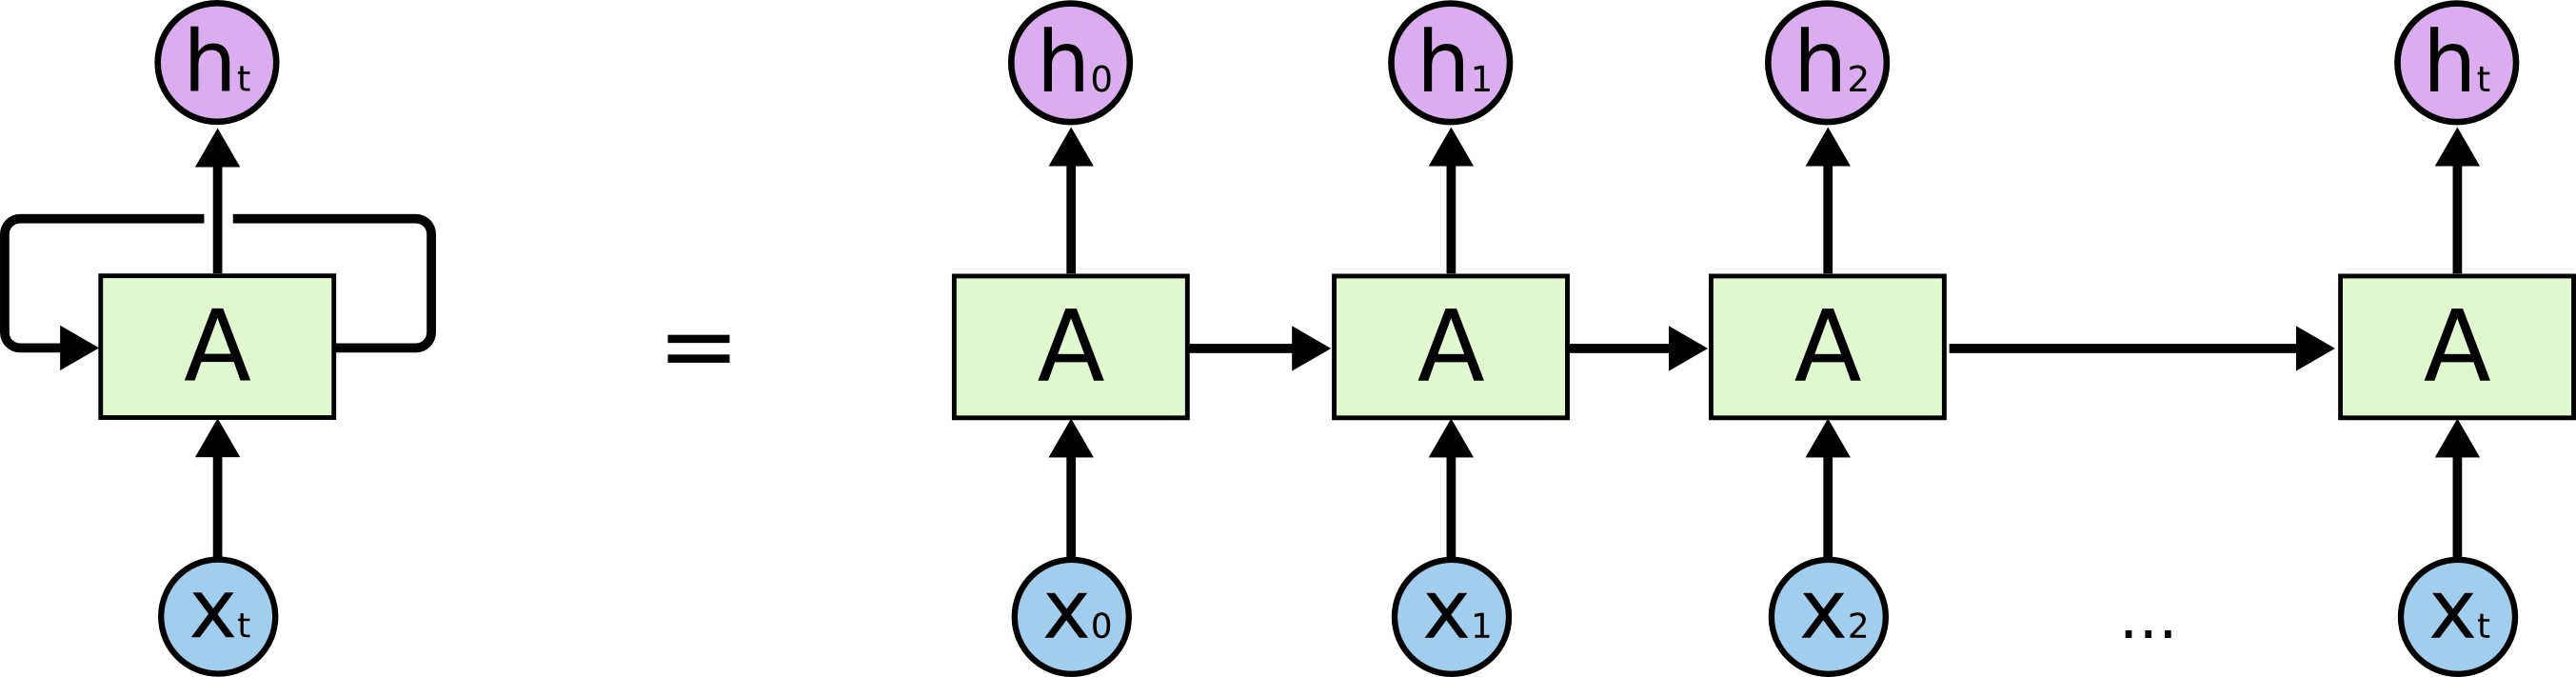
\includegraphics[width=\linewidth]{RNN-unrolled.png}
  \caption{Unrolled unit of a RNN network.   source: https://medium.com/deep-math-machine-learning-ai/chapter-10-1-deepnlp-lstm-long-short-term-memory-networks-with-math-21477f8e4235}
  \label{fig:RNN Unrolled}
\end{figure}


In a full RNN, there are usually many layers of these units connected together to create more complicated functions of sequential data. The architecture can get complicated but it is important the keep in mind that the architecture is simply one big compositional functional approximation. More specifically RNNs can be described as a high-dimensional, hierarchical, differentiable, functional approximator.\\

\noindent Lets break down that definition.
\begin{enumerate}
  \item High Dimensional - rather than dealing with observations explicitly like in the regression case, deep models like RNN, encode the observations, into a higher dimensional latent space.
  \item Hierarchical - each hidden node in a RNN network is passed to another node in the next layer such that each successive layer can work with information processed by the previous layers.
  \item Differentiable - all the components of RNNs must be differentiable, so you can understand which way to move parameters in the network with respect to the loss for a certain input. This results in long, complicated strings of chain rule for deep networks. In regression, the parameters' relationship to the least square loss was much more clear. $(X^TX)^{-1}X^Ty$ where the parameters of regression are deterministically composed of a term involving the covariance of the input data,$(X^TX)$.
  \item Functional Approximators - at the end of the day, the RNN is approximating a function that you cannot easily construct nor directly optimize with an approximated nonlinear function which can be optimized through backpropogation.
\end{enumerate}

\noindent RNNs use backpropogation to update parameters inside each RNN module with respect to the loss. However, information from long term dependencies cause the gradients with respect to those inputs to diminish over time. This would be less than ideal if we are predicting stock prices and a good predictor for tomorrow is the stock price a month ago. We need too handle the gradients with more care, thus introducing LSTM networks.

\section{Demystifying LSTM}

At a high level, LSTM Networks are just like RNN networks. They are a high-dimensional, hierarchical, differentiable, functional approximators. However, this time, as we zoom in, each module in the network is more complex - adding gating mechanisms (more nonlinearities) to persist gradients over longer periods of time. Lets now decompose this LSTM block with reference to the statistics framework we set up.\\

\begin{figure}
  \includegraphics[width=\linewidth]{lstm.png}
  \caption{One module of an LSTM network.  source: https://medium.com/deep-math-machine-learning-ai/chapter-10-1-deepnlp-lstm-long-short-term-memory-networks-with-math-21477f8e4235}
  \label{fig:LSTM Module}
\end{figure}

\noindent Defining terms and relationships:\\

\noindent $X_t$ = Current input vector\\
$\sigma$ = Sigmoid layer\\
tanh = non linear tanh layer\\
$H_{t-1}$ = last LSTM unit output\\
$C_{t-1}$ = last LSTM unit memory\\
$C_t$ = current unit memory\\
$H_t$ = current unit output\\

\noindent$f_t = \sigma(X_t * U_t + H_{t-1} * W_f)$\\
$\bar{C_t} = tanh(X_t * U_c + H_{t-1} * W_c)$\\
$I_t = \sigma(X_t * U_i + H_{t-1} * W_i)$\\
$O_t = \sigma(X_t * U_o + H_{t-1} * W_o)$\\

\noindent $C_t = f_t * C_{t-1} + I_t * \bar{C_t}$\\
$H_t = O_t * tanh(C_t)$\\
where W,U = weight vectors for forget gates,"*" is element-wise multiplication and "+" is element-wise addition\\

\noindent At first, this notation is a little scary, but this LSTM unit is just an ensemble of regression-like functions passed through non linear functions. Let us just follow the path the input takes through this cell. \\

\noindent $X_t$ is first weighted by 4 weight matrices. Each resulting term is added to the previous hidden state weighted by different weight matrices. This sum, $X_t*U+H_{t-1}*W$, can be thought of as a second order regression on these two states, $\beta_1X_t+\beta_2H_{t-1}$, only $H_{t-1}$ is a latent representation of previous inputs, rather, where $H_{t-1} = O_t * tanh(f_{t-1} * C_{t-2} + I_{t-1} * \bar{C_{t-1}})$ Explaining what the cell memory, $C_t$ is a little more tricky. $C_t$ can be thought of as a prior for our LSTM network built up from weights learned from data. Like in HMMs where we could factor $p_{Y_i|X_{i}}(y_i|x_{i})$ into our model to improve tracking a hidden state, our LSTM network learns this prior from data. Only, now the prior observation model is dynamic, changing with the hidden state $H_t$. The above equations yield $C_t = \sigma(X_t * U_t + H_{t-1} * W_f) * C_{t-1} + I_t * \bar{C_t}$ so $C_t$ is coupled with the movements of the hidden state. Many cite this as the reason LSTMs are such powerful models: The cell memory or the "observation model" in HMM land, can change over time to fit more complicated sequential processes.\\

\noindent Despite all the intricate details of the model, the process of training an LSTM network is pretty easy, yet more open ended.
\begin{enumerate}
  \item Define model architecture (no good groundwork for how to do this)
  \item Specify loss function (same as judgment criterion in regression)
  \item Evaluate and tune hyperparamters (no rules for how to evaluate hyperparameters other than
  trial and error)
\end{enumerate}

\section{Experiments}
In this section we compare regression to LSTM networks. We use the popular Keras deep learning library for creating LSTM networks. For these experiments we limit the scope to technical analysis (using the time series itself to forecast). For this reason, we leave out HMM, which require more hidden state design (known as fundamental analysis in finance) making it less comparable to the other methods. Furthermore, we predict known random processes so we can control out any biases brought about by specific datasets.

\subsection{Preparing data and Visualizing Data}
Here, we create the a noisy sinusoidal process and prepare it for modeling.  We don't need to split up into training, validation and testing sets as our models are known and stationary (population is similar to empirical samples).
\begin{Schunk}
\begin{Sinput}
> library(keras)
> generate_data<-function(n=10000,t = seq(0,4*pi,,1000),b=5, noise) {
+     a = array(data = numeric(n), dim = c(n, 1, 1))
+     a[,1,1]=sin(b*t)+noise
+     return(a)
+ }
> set.seed(1)
> n=1000
> y1 = generate_data(n=n,noise = rnorm(n))
> y1_scaled <- scale(y1,center = mean(y1), scale = sd(y1))
> plot(seq(length(y1_scaled)), y1_scaled, t="l", ylim=range(y1)*1.2)
> legend("top", legend=c("data"), col=1, lty=1, ncol=2, bty="n")
\end{Sinput}
\end{Schunk}
\includegraphics{18S096-001}
\subsection{Regression}
To echo the anlaysis done in the section on Regression, we implement the autoregressive model (10th order) with linear regression. Even though we know the model and can make our linear regression basis sinusodal, we pretend we do not have access to the underlying model.
\begin{Schunk}
\begin{Sinput}
> source("util.R")
> y0=y1
> T <- length(y0)
> index.lag0<-c(11:T)
> y0.lag0=y0[index.lag0]
> y0.lag1=y0[index.lag0-1]
> y0.lag2=y0[index.lag0-2]
> y0.lag3=y0[index.lag0-3]
> y0.lag4=y0[index.lag0-4]
> y0.lag5=y0[index.lag0-5]
> y0.lag6=y0[index.lag0-6]
> y0.lag7=y0[index.lag0-7]
> y0.lag8=y0[index.lag0-8]
> y0.lag9=y0[index.lag0-9]
> y0.lag10=y0[index.lag0-10]
> ones=0*y0.lag0+1
> xmat=cbind(ones,y0.lag1,y0.lag2,y0.lag3,y0.lag4,y0.lag5,y0.lag6,y0.lag7,y0.lag8,y0.lag9,y0.lag10)
> y0.arima.regress<-lm(y0.lag0~.,data = data.frame(xmat))
> print(y0.arima.regress$coefficients)
\end{Sinput}
\begin{Soutput}
 (Intercept)         ones      y0.lag1      y0.lag2      y0.lag3      y0.lag4 
-0.008769154           NA  0.086438945  0.082331483  0.082779311  0.070711441 
     y0.lag5      y0.lag6      y0.lag7      y0.lag8      y0.lag9     y0.lag10 
 0.112883016  0.015530022  0.121194759  0.067420018  0.089850015  0.063158707 
\end{Soutput}
\begin{Sinput}
> residuals = y0.arima.regress$residuals
> print("absolute error loss (MAE) L1 loss:")
\end{Sinput}
\begin{Soutput}
[1] "absolute error loss (MAE) L1 loss:"
\end{Soutput}
\begin{Sinput}
> print(mean(abs(residuals)))
\end{Sinput}
\begin{Soutput}
[1] 0.8692543
\end{Soutput}
\begin{Sinput}
> print("absolute error loss (MSE): L2  loss")
\end{Sinput}
\begin{Soutput}
[1] "absolute error loss (MSE): L2  loss"
\end{Soutput}
\begin{Sinput}
> print(mean(residuals**2))
\end{Sinput}
\begin{Soutput}
[1] 1.199611
\end{Soutput}
\begin{Sinput}
> print("absolute error loss (MSE): L1  loss for common sense metric")
\end{Sinput}
\begin{Soutput}
[1] "absolute error loss (MSE): L1  loss for common sense metric"
\end{Soutput}
\begin{Sinput}
> print(mean(abs(diff(y0))))
\end{Sinput}
\begin{Soutput}
[1] 1.2054
\end{Soutput}
\end{Schunk}
We show various residual errors for this regression model. Our MSE L2 loss is 1.19961. A good indicator for how well the model is modeling the signal part of the process (sinusoid) is comparing the MSE to the variance of the additive noise which is 1. For the conservative 1 step forward forecast, the model captures the signal pretty well. However, it barley outperforms the common sense estimator predicting the value at timestep n+1 to be the value at timestep n.
\begin{Schunk}
\begin{Sinput}
> propgate_forward_regress<-function(y,coeff){
+   line = rep(0,length(y)+1)
+   for(i in length(coeff)+1:length(y)){
+     line[i+1] = c(y[(i-9):i])%*%c(coeff)
+   }
+   return(line)
+ }
> weights = matrix(y0.arima.regress$coefficients)[3:12]
> predictions = propgate_forward_regress(y0,rev(weights))
> x=seq(length(predictions))
> plot(x,y0[1:length(predictions)],type="l",col="red",ylim = (1.2*range(y1)))
> lines(x,predictions,type = "l",col="green")
\end{Sinput}
\end{Schunk}
\includegraphics{18S096-003}
\\
From the graph, the green line is the predicted for the 1 step forecasting. You can see that this model is getting "pulled" by the noise, distracting it from the signal.
In this model and our previous regression analysis, we restricted ourselves to regressing on linear basis functions. With nonlinear kernels however, our modeling capabilities become much more powerful, but we still stay in the realm of least squares regression on a linear basis for clarity! 

\begin{Schunk}
\begin{Sinput}
> f_norm<-function(x){dnorm(x)}
> residual = y0[1:length(predictions)]-predictions
> hist(residual,freq = FALSE)
> curve(f_norm,add=TRUE,col='blue')
> print(sum(log(dnorm(na.omit(residual)))))
\end{Sinput}
\begin{Soutput}
[1] -1517.482
\end{Soutput}
\end{Schunk}
\includegraphics{18S096-004}
\\We also quickly take a look at the distribution of the residual errors in this model. The errors look pretty gaussian. The log liklihood of the data under the gaussian assumption is also shown. Now lets see how LSTMs perform on this simple time varying process.

\subsection{LSTM}
\begin{Schunk}
\begin{Sinput}
> batch_size =10
> model <- keras_model_sequential()
> model %>%
+   layer_lstm(units = 5, input_shape = list(10, 1), batch_size = batch_size,return_sequences = TRUE, stateful = TRUE) %>% 
+   layer_lstm(units = 5, return_sequences = FALSE, stateful = TRUE) %>% 
+   layer_dense(units = 1)
> model %>% compile(loss = 'mse', optimizer = 'rmsprop')
> summary(model)
\end{Sinput}
\begin{Soutput}
Model
________________________________________________________________________________
Layer (type)                        Output Shape                    Param #     
================================================================================
lstm_1 (LSTM)                       (10, 10, 5)                     140         
________________________________________________________________________________
lstm_2 (LSTM)                       (10, 5)                         220         
________________________________________________________________________________
dense_1 (Dense)                     (10, 1)                         6           
================================================================================
Total params: 366.0
Trainable params: 366
Non-trainable params: 0.0
________________________________________________________________________________
\end{Soutput}
\end{Schunk}
Here we construct a LSTM model with two layers each with 5 units. Compared to our 10 parameter regression model, this model seems like overkill, but we proceed to see how it performs.
We now construct a similar matrix for the regression case we covered earlier. But this matrix will now act as a training data matrix with multiple samples of shifted time series. We train each sample to predict the n+1 forecast.
\begin{Schunk}
\begin{Sinput}
> mat=cbind(y0.lag0,y0.lag1,y0.lag2,y0.lag3,y0.lag4,y0.lag5,y0.lag6,y0.lag7,y0.lag8,y0.lag9)
> train = array(NA, dim=c(990, 10, 1))
> train[,,1] =mat
> label = y0.lag10
> history <- model %>% fit(train, label, batch_size =  batch_size,
+                 epochs = 3, verbose = 1, shuffle = FALSE)
> #plot.new()
> plot(history)
> #title(main= "Training Loss Over Time (MSE)")
\end{Sinput}
\end{Schunk}
\includegraphics{18S096-006}
\\In just 3 epochs, our model can drastically decreased the average MSE loss.

\begin{Schunk}
\begin{Sinput}
> predicted_output <- model %>% predict(train,batch_size=batch_size)
> model %>% evaluate(train,label,batch_size=batch_size)
\end{Sinput}
\begin{Soutput}
    loss 
1.084858 
\end{Soutput}
\begin{Sinput}
> x = seq(length(predicted_output))
> plot(x,label,type = "l", xlab = '',col='red')
> lines(x,predicted_output,type="l", xlab = '',col='green')
\end{Sinput}
\end{Schunk}
\includegraphics{18S096-007}
\begin{Schunk}
\begin{Sinput}
> f_norm<-function(x){dnorm(x)}
> residual = predicted_output-label
> hist(residual,freq = FALSE)
> curve(f_norm,add=TRUE,col='blue')
> print(sum(log(dnorm(residual))))
\end{Sinput}
\begin{Soutput}
[1] -1446.759
\end{Soutput}
\end{Schunk}
\includegraphics{18S096-008}
\\The Mean Square Error Loss is less than the regression loss. So from this perspective, it has a lot more modeling power. Its ability to use nonlinear functions allow LSTMs to approximate sinusoidal functions much more accurately than a linear model. Additionally, the loss is pretty close to one. As mentioned earlier, a loss of 1 would correspond to perfectly capturing the sinusoidal signal, as the MSE would be the MSE of the random process which is the simply its unit variance. Looking at the distribution of the residual errors, the plot looks pretty guassian, just like the additive noise of the model. And under the gaussian model, the logliklihood of the errors are higher for the LSTM model!

It is important to take the power of LSTMs with a grain of salt. The large amount of parameters needed to model a process could lead to over fitting. More care would have to be taken in tuning hyperparamters on a more versatile dataset.

\section{References}

1.https://tensorflow.rstudio.com/blog/time-series-forecasting-with-recurrent-neural-networks.html\\
2. https://datamarket.com/data/list/?q=cat:ecc%20provider:tsdl\\
3.https://medium.com/deep-math-machine-learning-ai/chapter-10-1-deepnlp-lstm-long-short-term-memory-networks-with-math-21477f8e4235\\
4. 18.S096 2018 class notes

\end{document}
